%%%%%%%%%%%%%%%%%%%%%%%%%%%%%%%%%%%%%%%%%%%%%%%%%%%%%%%%
\documentclass[12pt,a4paper]{article}% 文档格式
\usepackage{ctex,hyperref}% 输出汉字
\usepackage{times}% 英文使用Times New Roman
%%%%%%%%%%%%%%%%%%%%%%%%%%%%%%%%%%%%%%%%%%%%%%%%%%%%%%%%
\title{\fontsize{18pt}{27pt}\selectfont% 小四字号,1.5倍行距
	{\heiti% 黑体 
    基于深度学习的自动化小行星搜索}}% 题目
%%%%%%%%%%%%%%%%%%%%%%%%%%%%%%%%%%%%%%%%%%%%%%%%%%%%%%%%
\author{\fontsize{12pt}{18pt}\selectfont% 小四字号,1.5倍行距
	{\fangsong% 仿宋
		孙畅,邹桐,周佳颖 }\\% 标题栏脚注
	\fontsize{10.5pt}{15.75pt}\selectfont% 五号字号,1.5倍行距
	{\fangsong% 仿宋
		(南京外国语学校,江苏省南京市玄武区北京东路30号)}}% 作者单位,“~”表示空格
%%%%%%%%%%%%%%%%%%%%%%%%%%%%%%%%%%%%%%%%%%%%%%%%%%%%%%%%
\date{}% 日期(这里避免生成日期)
%%%%%%%%%%%%%%%%%%%%%%%%%%%%%%%%%%%%%%%%%%%%%%%%%%%%%%%%
\usepackage{amsmath,amsfonts,amssymb}% 为公式输入创造条件的宏包
%%%%%%%%%%%%%%%%%%%%%%%%%%%%%%%%%%%%%%%%%%%%%%%%%%%%%%%%
\usepackage{graphicx}% 图片插入宏包
\usepackage{subfigure}% 并排子图
\usepackage{float}% 浮动环境,用于调整图片位置
\usepackage[export]{adjustbox}% 防止过宽的图片
%%%%%%%%%%%%%%%%%%%%%%%%%%%%%%%%%%%%%%%%%%%%%%%%%%%%%%%%
\usepackage{bibentry}
\usepackage{natbib}% 以上2个为参考文献宏包
%%%%%%%%%%%%%%%%%%%%%%%%%%%%%%%%%%%%%%%%%%%%%%%%%%%%%%%%
\usepackage{abstract}% 两栏文档,一栏摘要及关键字宏包
\renewcommand{\abstracttextfont}{\fangsong}% 摘要内容字体为仿宋
\renewcommand{\abstractname}{\textbf{摘\quad 要}}% 更改摘要二字的样式
%%%%%%%%%%%%%%%%%%%%%%%%%%%%%%%%%%%%%%%%%%%%%%%%%%%%%%%%
\usepackage{xcolor}% 字体颜色宏包
\newcommand{\red}[1]{\textcolor[rgb]{1.00,0.00,0.00}{#1}}
\newcommand{\blue}[1]{\textcolor[rgb]{0.00,0.00,1.00}{#1}}
\newcommand{\green}[1]{\textcolor[rgb]{0.00,1.00,0.00}{#1}}
\newcommand{\darkblue}[1]
{\textcolor[rgb]{0.00,0.00,0.50}{#1}}
\newcommand{\darkgreen}[1]
{\textcolor[rgb]{0.00,0.37,0.00}{#1}}
\newcommand{\darkred}[1]{\textcolor[rgb]{0.60,0.00,0.00}{#1}}
\newcommand{\brown}[1]{\textcolor[rgb]{0.50,0.30,0.00}{#1}}
\newcommand{\purple}[1]{\textcolor[rgb]{0.50,0.00,0.50}{#1}}% 为使用方便而编辑的新指令
%%%%%%%%%%%%%%%%%%%%%%%%%%%%%%%%%%%%%%%%%%%%%%%%%%%%%%%%
\usepackage{url}% 超链接
\usepackage{bm}% 加粗部分公式
\usepackage{multirow}
\usepackage{booktabs}
\usepackage{epstopdf}
\usepackage{epsfig}
\usepackage{longtable}% 长表格
\usepackage{supertabular}% 跨页表格
\usepackage{algorithm}
\usepackage{algorithmic}
\usepackage{changepage}% 换页
%%%%%%%%%%%%%%%%%%%%%%%%%%%%%%%%%%%%%%%%%%%%%%%%%%%%%%%%
\usepackage{enumerate}% 短编号
\usepackage{caption}% 设置标题
\captionsetup[figure]{name=\fontsize{10pt}{15pt}\selectfont Figure}% 设置图片编号头
\captionsetup[table]{name=\fontsize{10pt}{15pt}\selectfont Table}% 设置表格编号头
%%%%%%%%%%%%%%%%%%%%%%%%%%%%%%%%%%%%%%%%%%%%%%%%%%%%%%%%
\usepackage{indentfirst}% 中文首行缩进
\usepackage[left=2.50cm,right=2.50cm,top=2.80cm,bottom=2.50cm]{geometry}% 页边距设置
\renewcommand{\baselinestretch}{1.5}% 定义行间距(1.5)
%%%%%%%%%%%%%%%%%%%%%%%%%%%%%%%%%%%%%%%%%%%%%%%%%%%%%%%%
\usepackage{fancyhdr} %设置全文页眉、页脚的格式
\pagestyle{fancy}
\hypersetup{colorlinks=true,linkcolor=black}% 去除引用红框,改变颜色
%%%%%%%%%%%%%%%%%%%%%%%%%%%%%%%%%%%%%%%%%%%%%%%%%%%%%%%%


\begin{document}% 以下为正文内容

\begin{titlepage}
    \begin{flushleft}
        \fontsize{22pt}{40pt}\selectfont
        参赛队员姓名:\underline{孙畅,邹桐,周佳颖} \\
        中学:\underline{南京外国语学校}\\
        省份:\underline{江苏省}\\
        国家/地区:\underline{中国/南方赛区}\\
        指导教师姓名:\underline{史镨镭}\\
        指导教师单位:\underline{南京外国语学校}\\
        论文题目:\underline{基于深度学习的自动化小行星搜索}
    \end{flushleft}
\end{titlepage}

\maketitle% 产生标题,没有它无法显示标题
%%%%%%%%%%%%%%%%%%%%%%%%%%%%%%%%%%%%%%%%%%%%%%%%%%%%%%%%
\lhead{}% 页眉左边设为空
\chead{}% 页眉中间设为空
\rhead{}% 页眉右边设为空
\lfoot{}% 页脚左边设为空
\cfoot{\thepage}% 页脚中间显示页码
\rfoot{}% 页脚右边设为空
%%%%%%%%%%%%%%%%%%%%%%%%%%%%%%%%%%%%%%%%%%%%%%%%%%%%%%%%
\begin{abstract}
    \fangsong 小行星观测和搜索是人类确保地球生存环境安全的关键一环,对我们了解太阳系的起源和演化有重要意义。然而,现有的观测图像搜索方法往往存在准确率偏低、可迁移性和延展性不足等问题,存在较大的局限性。本文提出使用深度学习中的迁移学习方法,利用哈勃空间望远镜公开数据建立标记数据集和进行训练,实现高精度的自动化小行星搜索流水线。经过实验,我们实现了最高准确率92.24\%,最大召回率91.25\%,效果令人满意。
\end{abstract}

\begin{adjustwidth}{1.06cm}{1.06cm}
    \fontsize{10.5pt}{15.75pt}\selectfont{\heiti{关键词:}\fangsong{小行星、深度学习、卷积神经网络、哈勃天文望远镜}}\\
\end{adjustwidth}

\newpage

\tableofcontents

\newpage

\section{引言}

小行星(Figure 1),一般指太阳系内的一类天体。该类天体类似行星环绕太阳运动,但体积和质量比行星小得多。小行星一般被认为是由太阳系形成时期的微行星演变而来,是目前发现数量最多的太阳系天体。

了解小行星的位置和轨道参数细节,对于人类在地球上的生存安全有极为重要的意义。1994年,苏梅克-列维九号彗星在分裂成21颗碎片后撞击木星,其中最大的一颗碎片直径达35公里,产生了明显的撞击坑。据估计,这次撞击相当于10亿颗原子弹同时爆炸的当量,对木星大气的影响直到三个月后才基本恢复。如果这样的撞击发生在地球上,将会对地球大气产生极为显著的影响。自此之后,IAU建立起完备的小行星观测、报备、核验系统,确认了相当数量的小行星,大大增加了我们对于地球所处的宇宙环境的了解。

\begin{figure}[H]% 插入一张图片,H表示浮动环境下的here
    \centering
    \begin{minipage}{0.7\textwidth}% 小页面尺寸,可自行调节
        \centering
        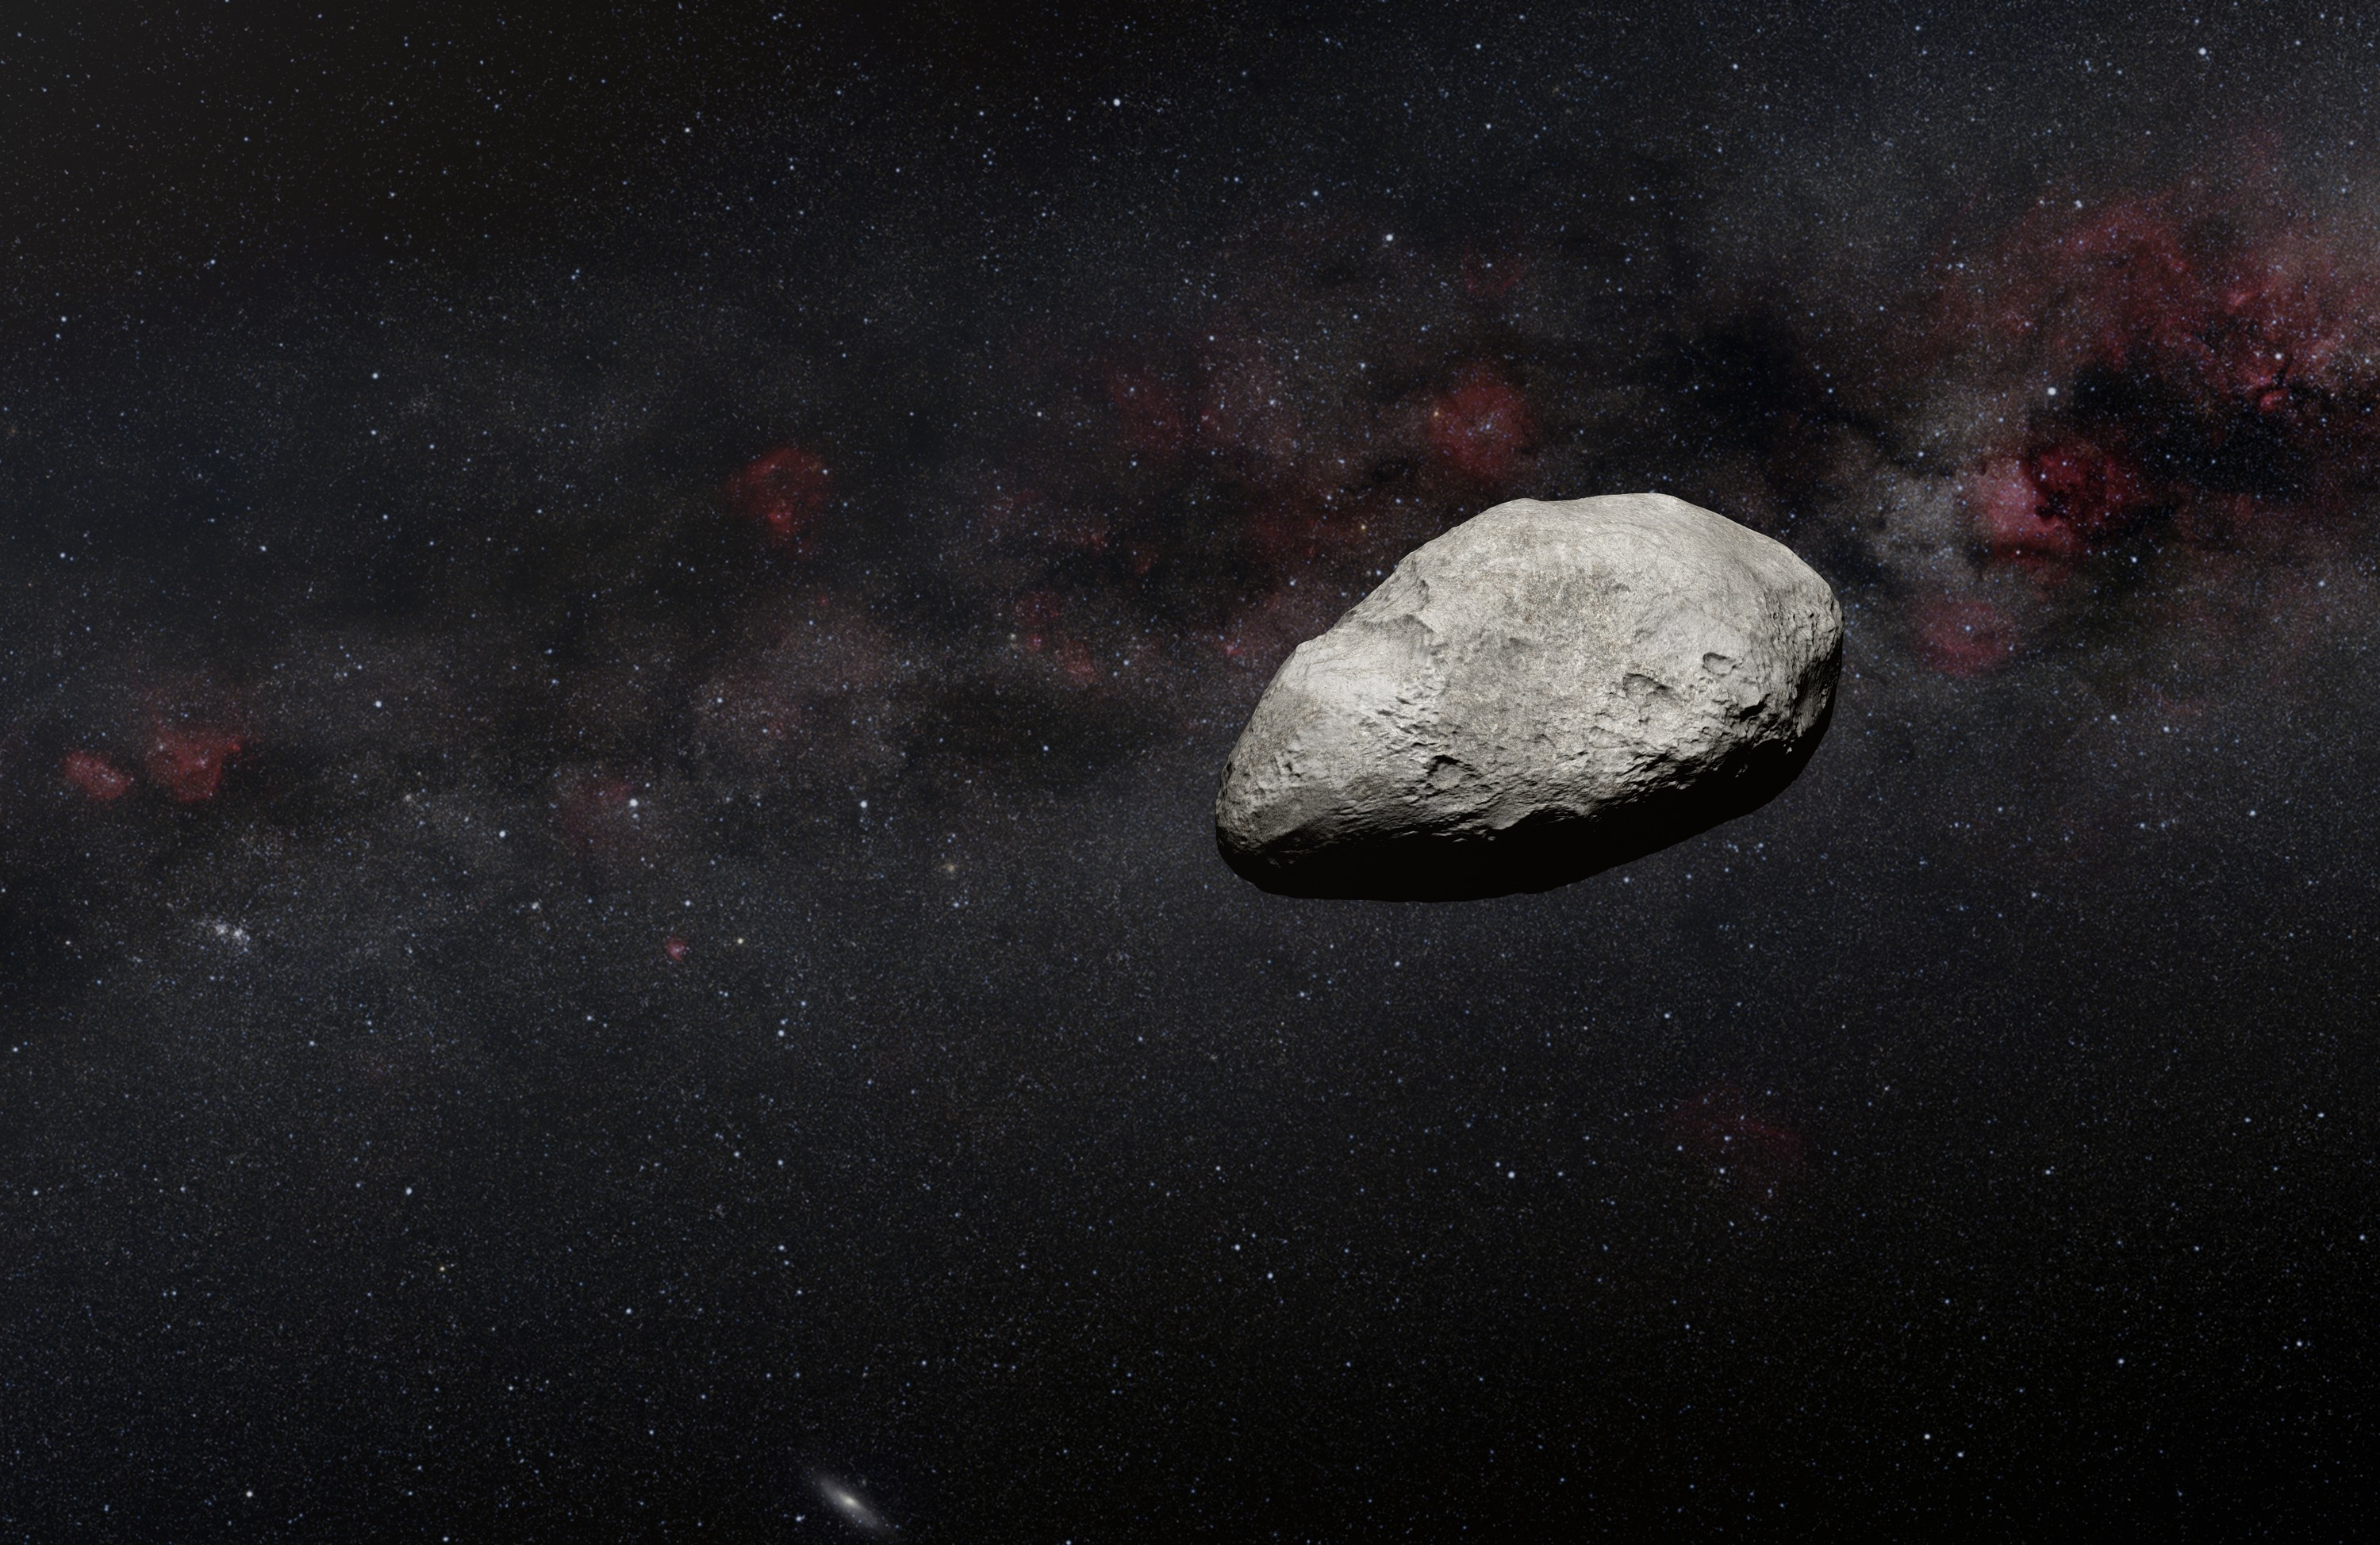
\includegraphics[width=1.0% 图片尺寸,可自行调节
            \textwidth]{asteroid}% 图片名称(图片需与tex文件在同一文件夹)
        \caption{\fontsize{10pt}{15pt}\selectfont 宇宙中的小行星示意图}% 图例
    \end{minipage}
\end{figure}

此外,包括小行星在内的太阳系小天体已成为人类了解太阳系的起源和发展的重要观测对象,对于人类揭开恒星系演化过程具有重要的意义。

截至目前,尽管已有相当多的太阳系内的小行星被发现、编号,仍然有大量的太阳系内小天体未被发现。世界各地的先进天文观测望远镜每天都在产生体量极大的观测数据,但是对于观测数据的处理、筛选、分析,仍然处于相对较低的水平。尽管在观测图像中存在相当数量的小行星踪迹,但由于拍摄出的照片体量相当大,且分析手段仍存在优化空间,所以仍可能有大量已经被拍摄到的小行星被我们忽略。

传统的小行星检测算法往往从小行星本身的物理特性出发,结合本观测站的观测条件,精心设计出特定的检测算法。然而,这类算法在不同的观测设备、观测方法和观测条件下迁移较为困难,且几乎所有的大型观测项目都不提供开源的小行星检测算法,在实际使用中存在较多限制。

一些大型观测项目逐渐意识到,在现有条件下,小行星观测数据往往存在图像分析能力不够、精确度不高的问题。于是,他们发起了一系列公众科学项目(如IASC和Hubble Asteroid Hunter),将望远镜产生的数据分发给参与项目的志愿者,借助社会力量来补充现有的数据分析手段。在这些公众科学项目中,参与项目的志愿者往往需要通过肉眼进行小行星检测,总体效率很低,且准确率无法保证。

针对以上问题,本文提出了使用深度学习方法来进行小行星搜寻工作。我们拟采取对经典的图像分类卷积神经网络进行微调的方法,实现高效、自动化小行星搜索工作。

\section{数据集构建}

\subsection{数据选取}

从观测的角度来说,地面观测通常受到昼夜更替、晴夜数量、夜天光情况和大气视宁度等因素的影响,对小行星的巡天观测条件比较苛刻。所以,选取拍摄质量更高的空间望远镜数据或将成为更好的选择。哈勃空间望远镜(Figure 2)作为部署在大气层外的先进光学望远镜,具有视场大、观测能力强、干扰较少、不受地表天气因素约束等优势,是进行小行星搜寻的良好器材。

\begin{figure}[H]% 插入一张图片,H表示浮动环境下的here
    \centering
    \begin{minipage}{0.7\textwidth}% 小页面尺寸,可自行调节
        \centering
        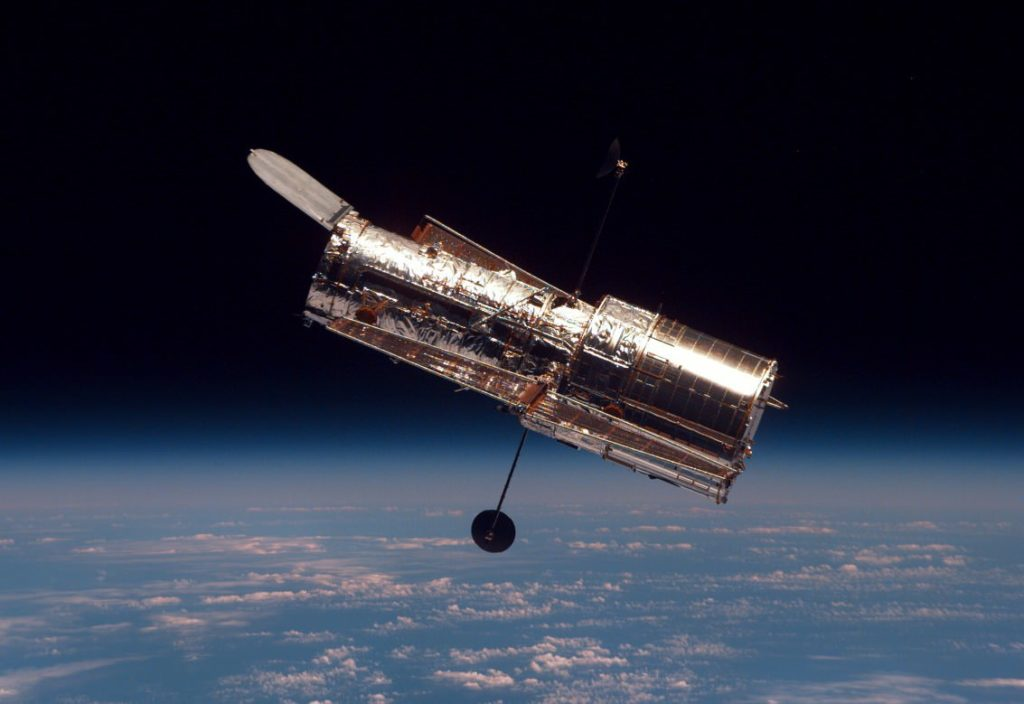
\includegraphics[width=1.0% 图片尺寸,可自行调节
            \textwidth]{hubble}% 图片名称(图片需与tex文件在同一文件夹)
        \caption{\fontsize{10pt}{15pt}\selectfont 哈勃空间望远镜}% 图例
    \end{minipage}
\end{figure}

为能够捕获到星际中微弱的电磁波信息,哈勃空间望远镜采用的是对指定区域的长时间曝光(平均每张照片曝光35分钟)的观测方法。在长时间曝光下,距离更远的恒星、星系、星云往往不会发生明显的位置变化,所以在图像中能够看到一个清晰的像。由于小行星是太阳系内天体,离望远镜距离要近很多,在一次曝光中会产生明显的位移,所以表现在照片上是一条线状轨迹。我们展示了几张哈勃望远镜的观测数据(Figure 3)。

哈勃团队为提高小行星搜索检测的准确率,发起了"Hubble Asteroid Hunter"公众科学项目。该项目借助公众力量和机器学习方法,发现了1701条小行星轨迹,其中670条被确认为已知的小行星。在项目结束后,哈勃团队公开了1701条数据的观测号、曝光时间、图像中小行星轨迹起始和终止位置等信息,为深度学习提供了较高质量的训练数据来源。该数据集是目前我们已知的唯一公开的标记数据集。

我们展示了哈勃团队提供的表格中的局部行列(Table 1)。表格中提供的小行星轨迹是使用天球坐标系上的RA(经度)和Dec(纬度)来描述的,单位是度,这是天文中常用的坐标系统,但是不适合我们进行进一步的深度学习训练。在后续处理中,我们将会把天球坐标系中的坐标转换成图像上的像素点坐标。

\begin{figure}[H]% 插入两张图片并且并排
    \centering
    \begin{minipage}{0.48\textwidth}
        \centering
        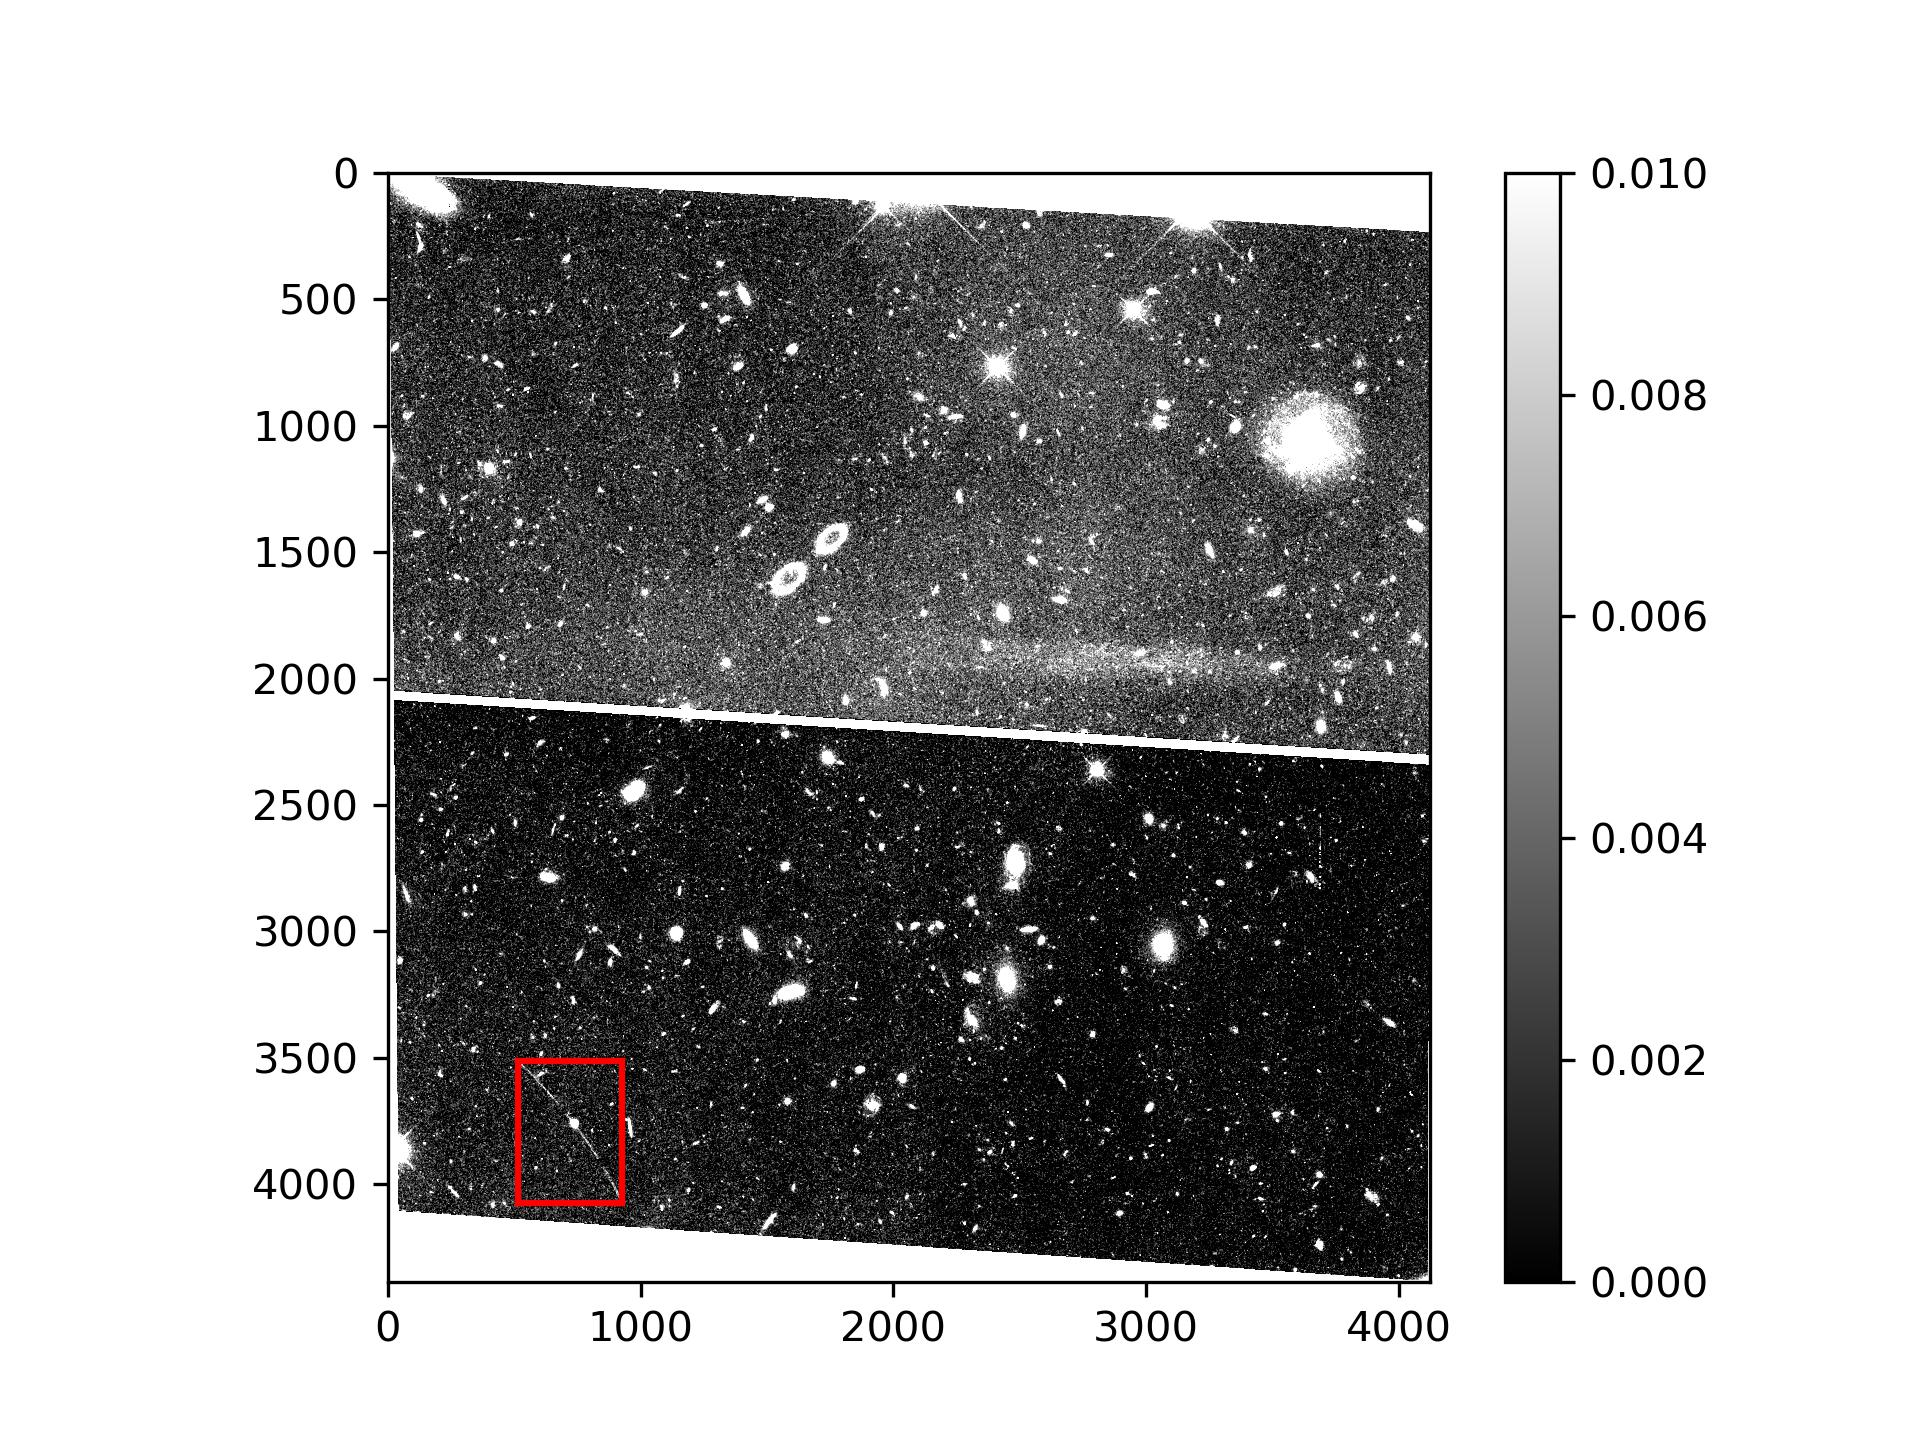
\includegraphics[width=0.83\textwidth]{fig71.jpg}

    \end{minipage}
    \hspace{0cm}% 图片间距
    \begin{minipage}{0.48\textwidth}
        \centering
        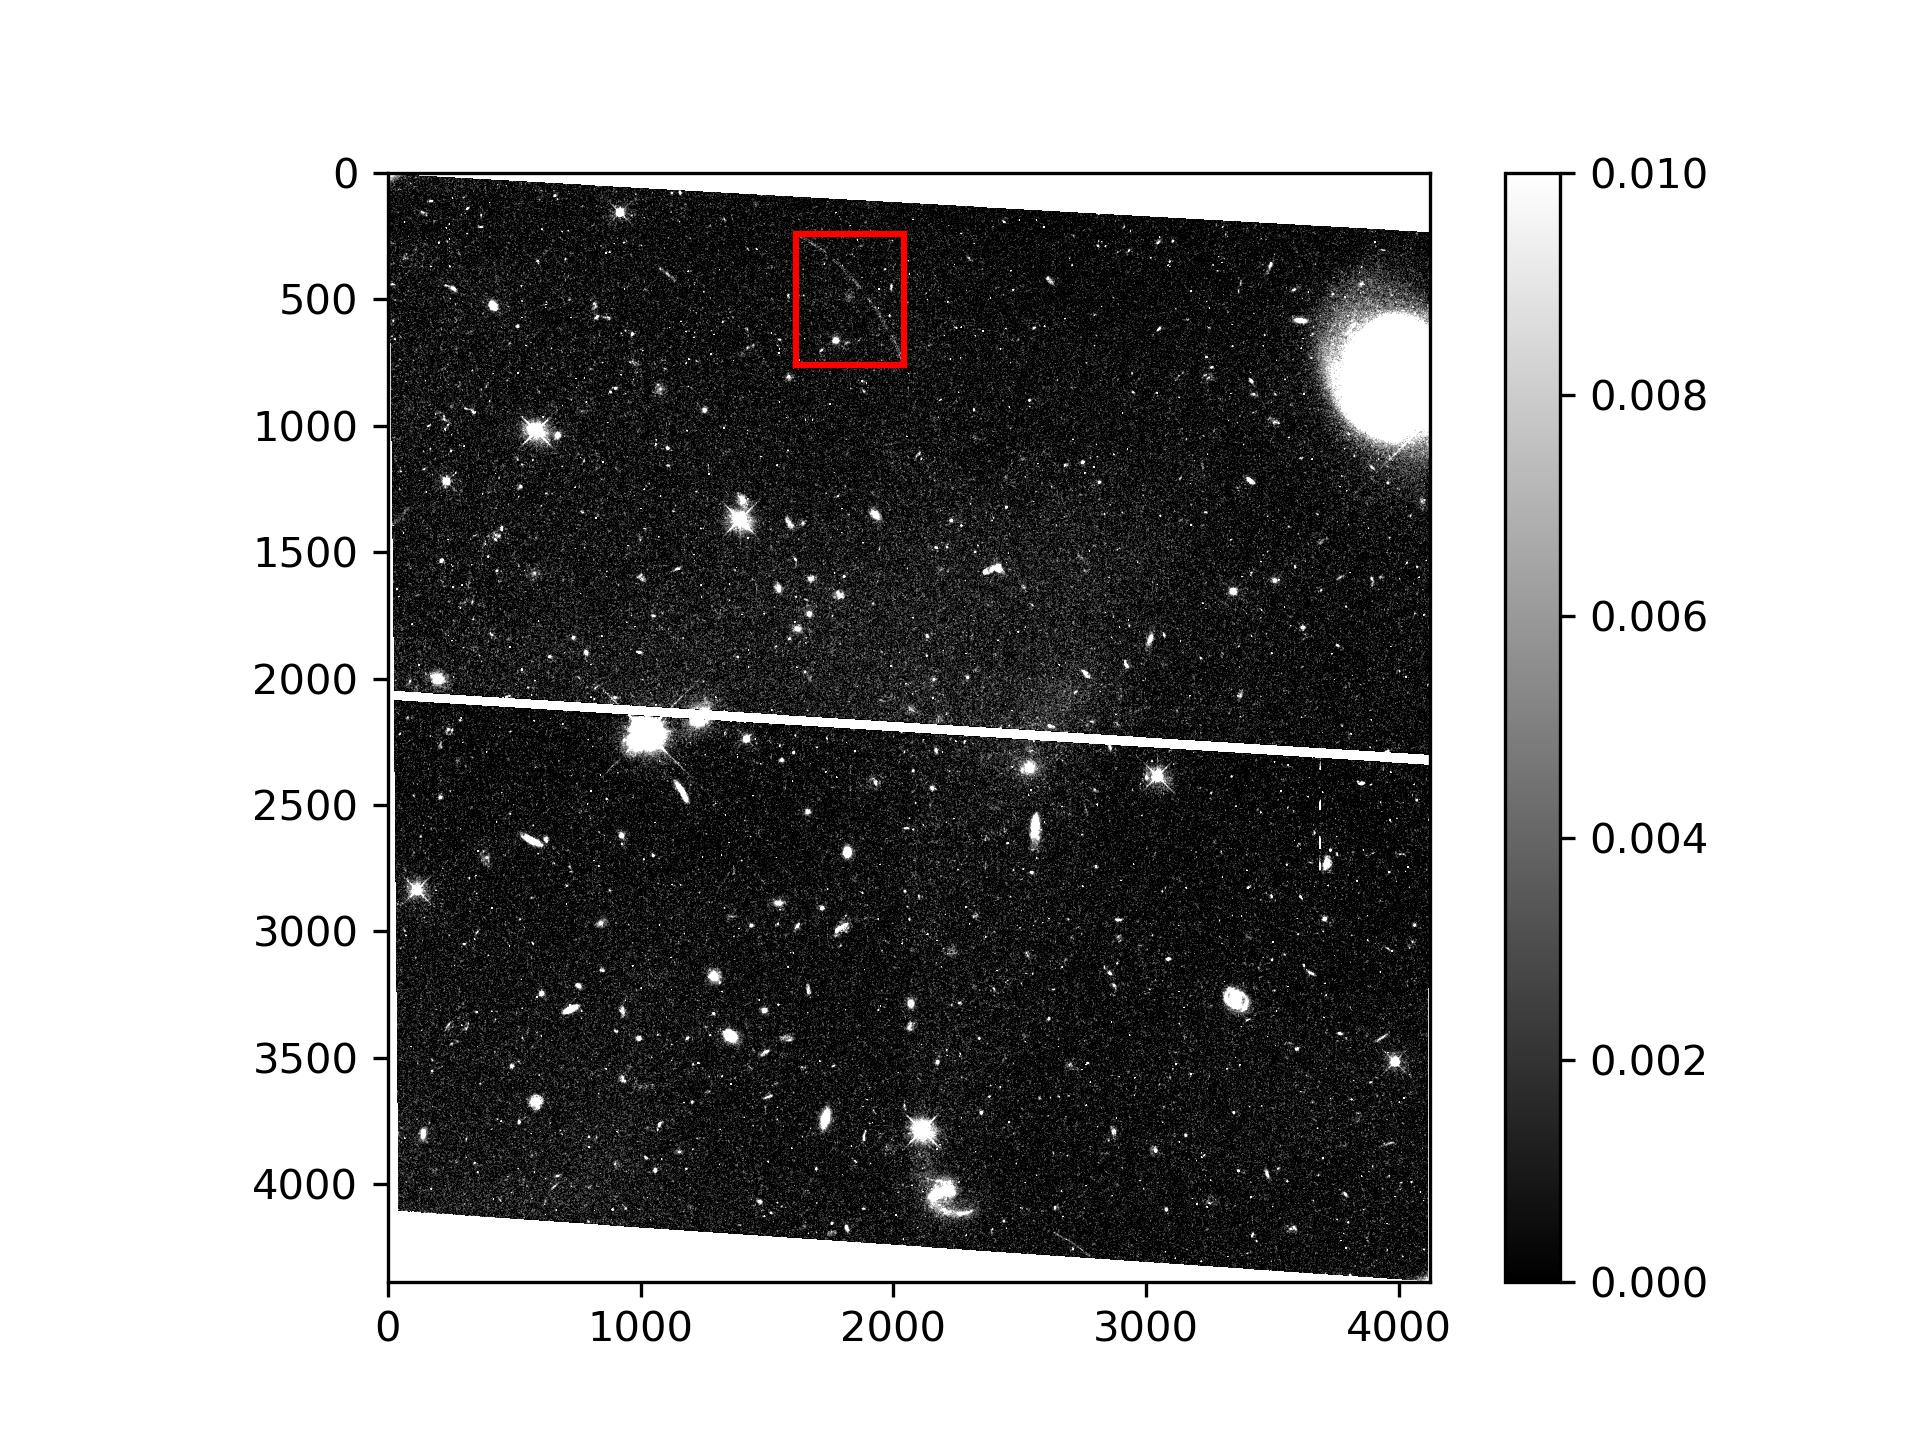
\includegraphics[width=0.83\textwidth]{fig167.jpg}
    \end{minipage}
    \begin{minipage}{0.48\textwidth}
        \centering
        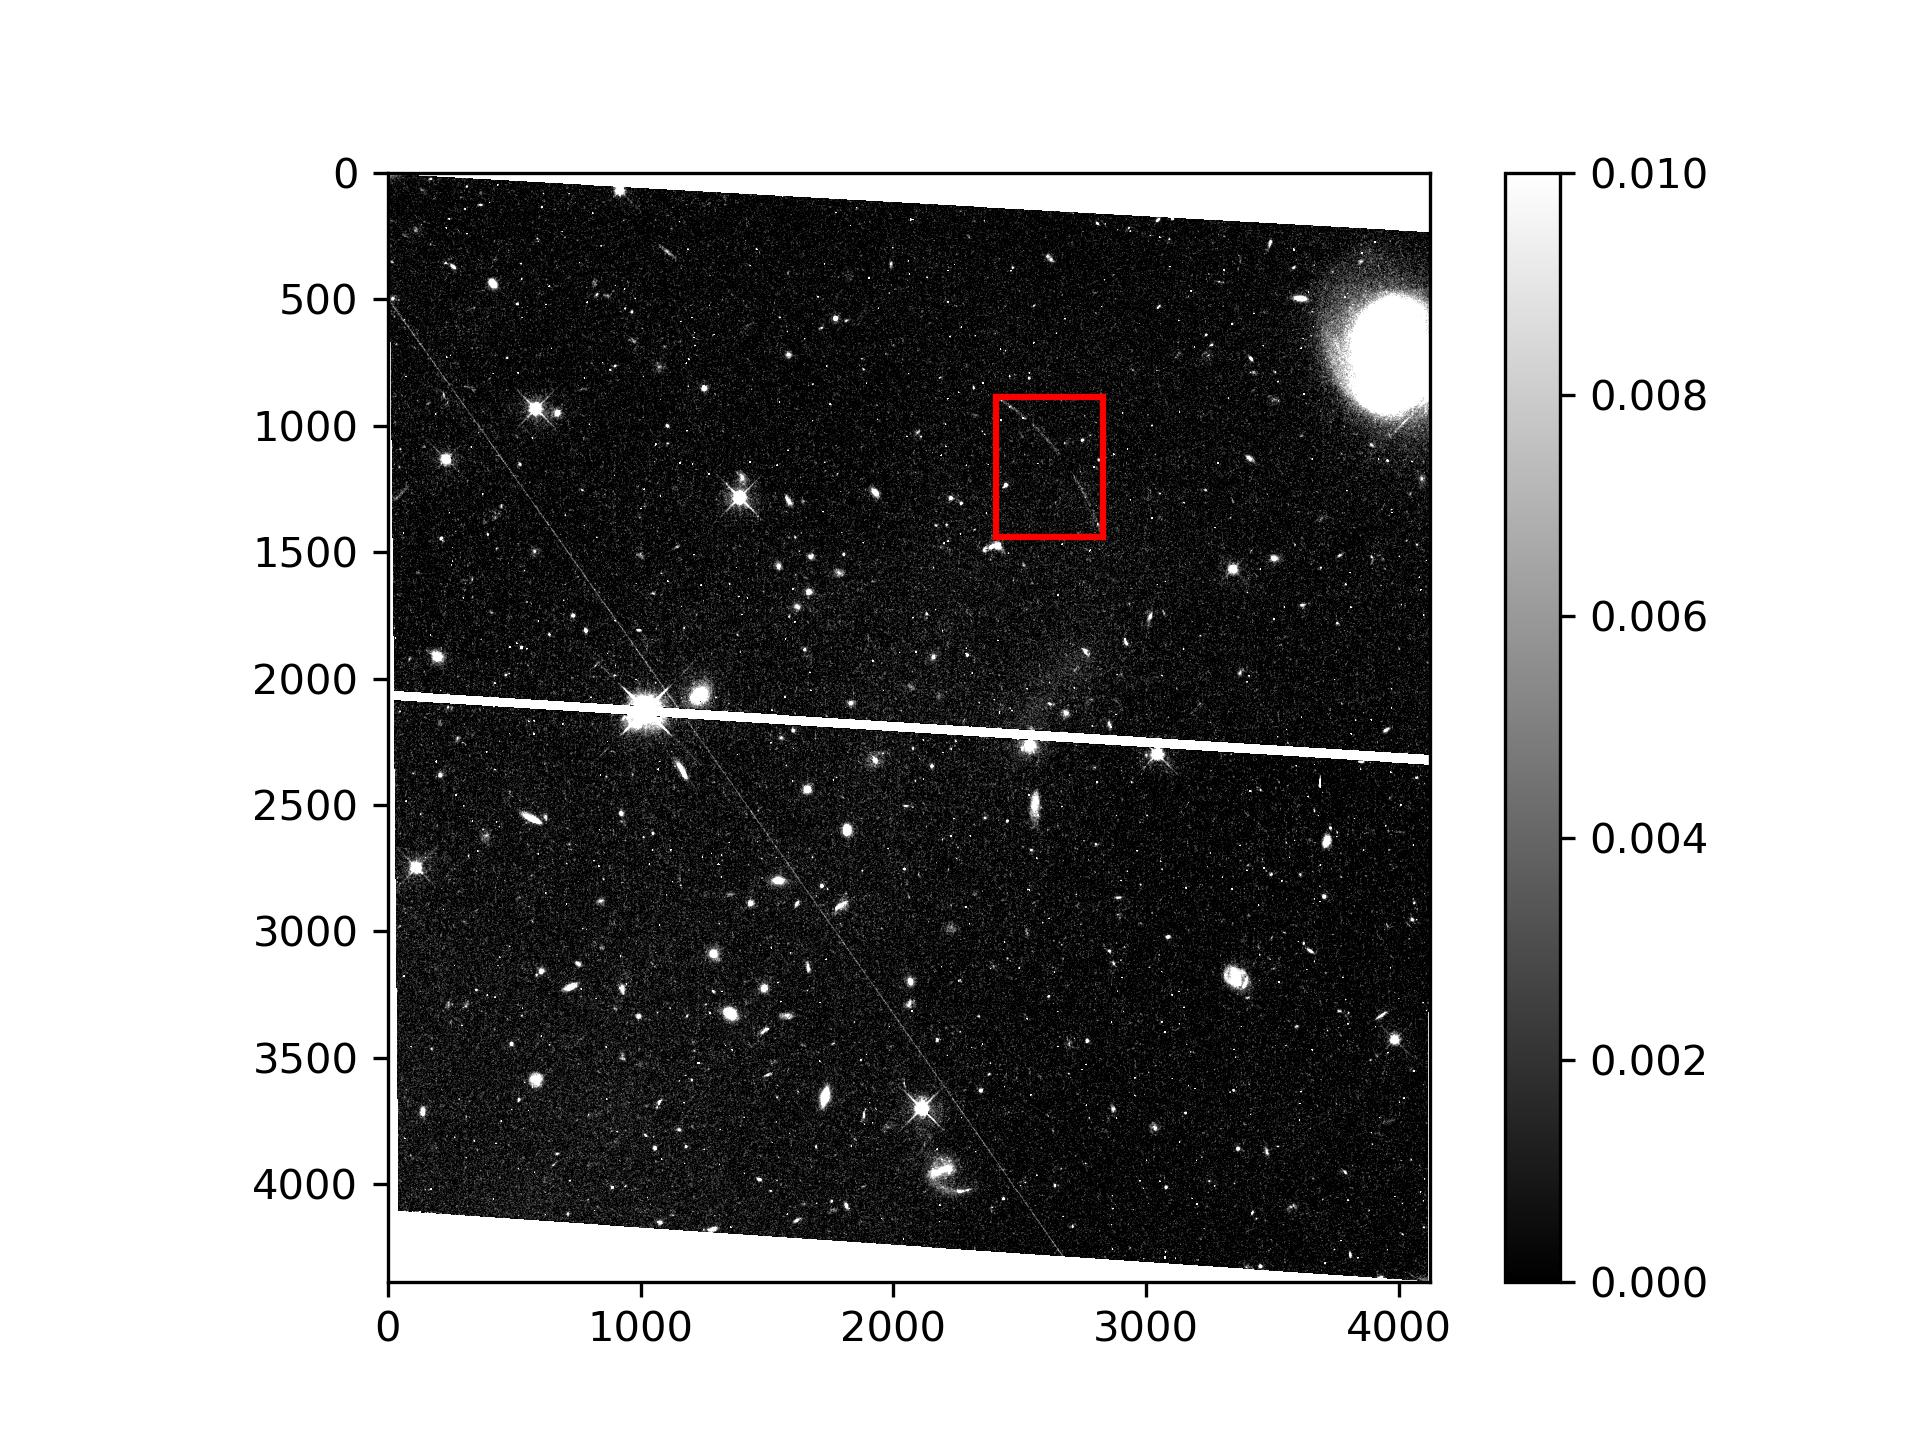
\includegraphics[width=0.83\textwidth]{fig168.jpg}
    \end{minipage}
    \hspace{0cm}% 图片间距
    \begin{minipage}{0.48\textwidth}
        \centering
        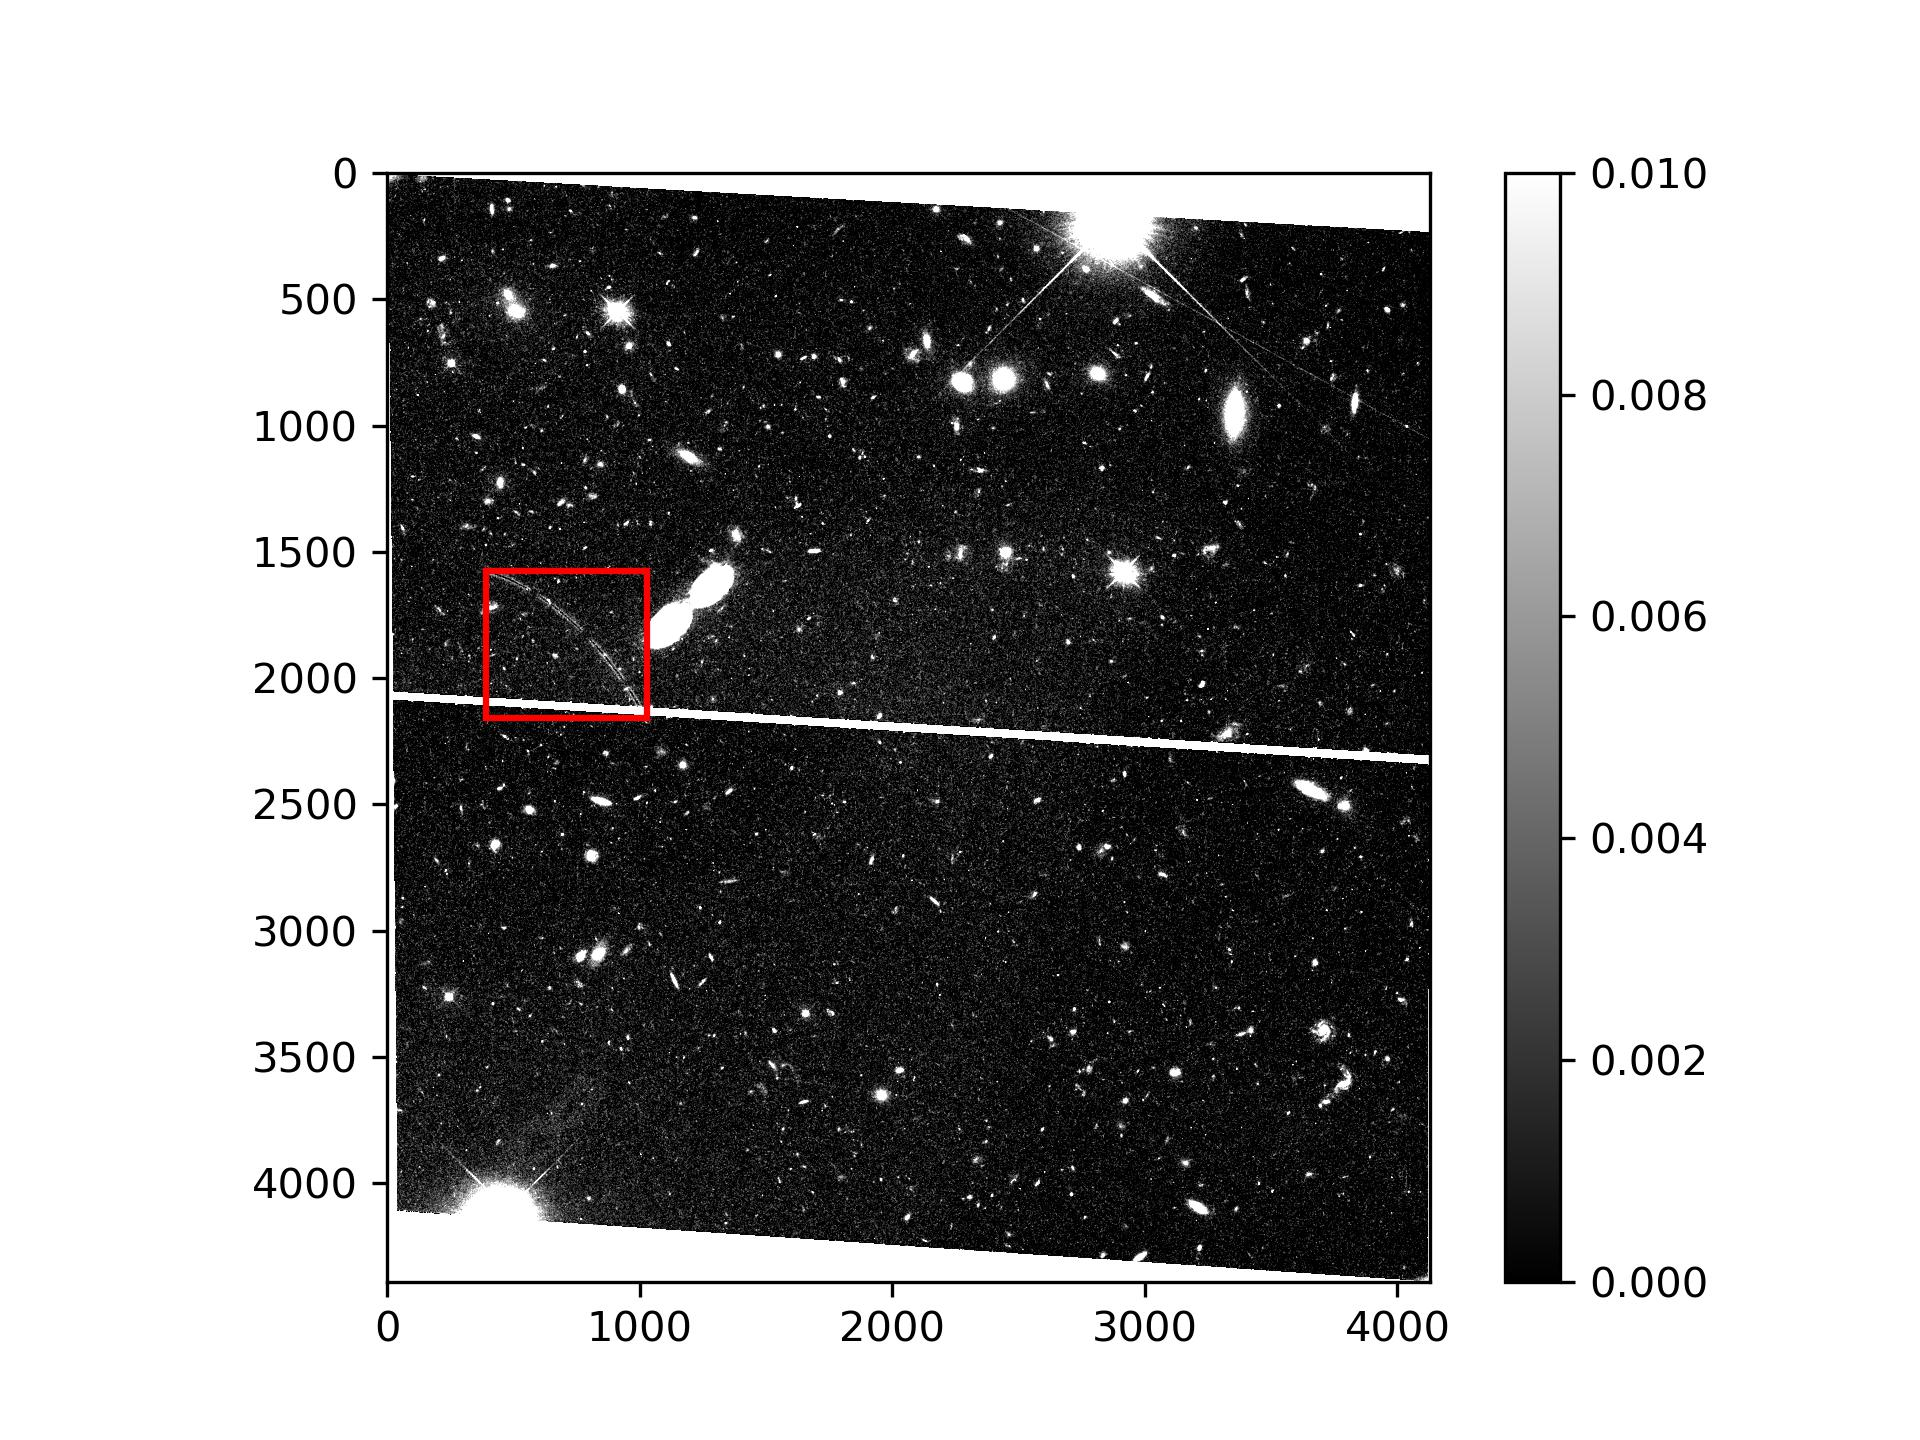
\includegraphics[width=0.83\textwidth]{fig223.jpg}
    \end{minipage}
    \caption{\fontsize{10pt}{15pt}\selectfont 哈勃观测图像与小行星轨迹样例}
\end{figure}




\begin{table}[H]% 插入表格
    \centering
    \caption{\fontsize{10pt}{15pt}\selectfont Hubble Asteroid Hunter数据集样例}
    \resizebox{\linewidth}{!}{
        \begin{tabular}{cccccc}
            \toprule[2pt]
            哈勃望远镜观测号  & 轨迹曝光时间(秒) & 轨迹起始位置RA    & 轨迹起始位置Dec  & 轨迹终止位置RA    & 轨迹终止位置Dec  \\

            \midrule
            ib1901010 & 2520.0    & 146.7329823 & 10.0969372 & 146.72596   & 10.0971402 \\
            ib2r03020 & 1340.0    & 57.8625451  & 28.3094616 & 57.866537   & 28.3105017 \\
            ib4801010 & 1772.0    & 135.3464886 & 18.2331854 & 135.3422318 & 18.2361665 \\
            ib4803010 & 3686.0    & 135.0326681 & 22.5615199 & 135.0202912 & 22.549794  \\
            ib4803020 & 2799.0    & 135.0172415 & 22.5440068 & 135.0042467 & 22.5320243 \\

            \bottomrule[2pt]
        \end{tabular}
    }
\end{table}

\subsection{图像预处理}

尽管该数据集提供了含有小行星照片的详细参数信息,但没有直接提供可以用于训练的哈勃望远镜观测照片。所以,我们设计了一套处理流程,实现由Python自动化完成数据批量下载、剪裁、导出并可视化等工作。以下是图像预处理的流程(Figure 4):

\begin{enumerate}[1.]% 列举时编号
    \item 读取哈勃团队提供的表格,获得指定观测号、小行星位置等关键信息;
    \item 使用Python中的astroquery第三方库,调用相关API,下载Mikulski Archive for Space Telescopes (MAST)数据库中指定观测号的数据\footnote{https://astroquery.readthedocs.io/en/latest/mast/mast.html};
    \item 提取天文标准数据格式FITS文件中的图像数据,处理成NumPy Array的格式;
    \item 对小行星轨迹标记的位置进行坐标转化。将原先天球坐标系统中的坐标转换成图像上的像素坐标,方便后续处理;
    \item 根据现有的小行星位置信息,引入x, y方向上的随机偏移,获取1000*1000像素点尺寸的包含小行星(positive类别)数据集。在这种构造方式下,可以在确保图像上保留全部或部分的小行星轨迹的同时,实现图像上的小行星轨迹随机出现,模拟真实应用场景下的图像。
    \item 将所有图像按照70/15/15的比例划分训练集(train)/验证集(val)/检测集(test)
\end{enumerate}

哈勃团队只提供了含有小行星的图像观测号,而没有提供不含小行星的观测号。为保证不包含小行星(negative类别)数据集的纯净性,我们从这些确保经过人工筛查的图像中,在远离小行星标记位置随机选取1000*1000像素点大小的图像,构成negative类别数据集。最终,我们数据集的大小为positive类别1696张,negative类别1586张。

\begin{figure}[H]% 插入一张图片,H表示浮动环境下的here
    \centering
    \begin{minipage}{1.0\textwidth}% 小页面尺寸,可自行调节
        \centering
        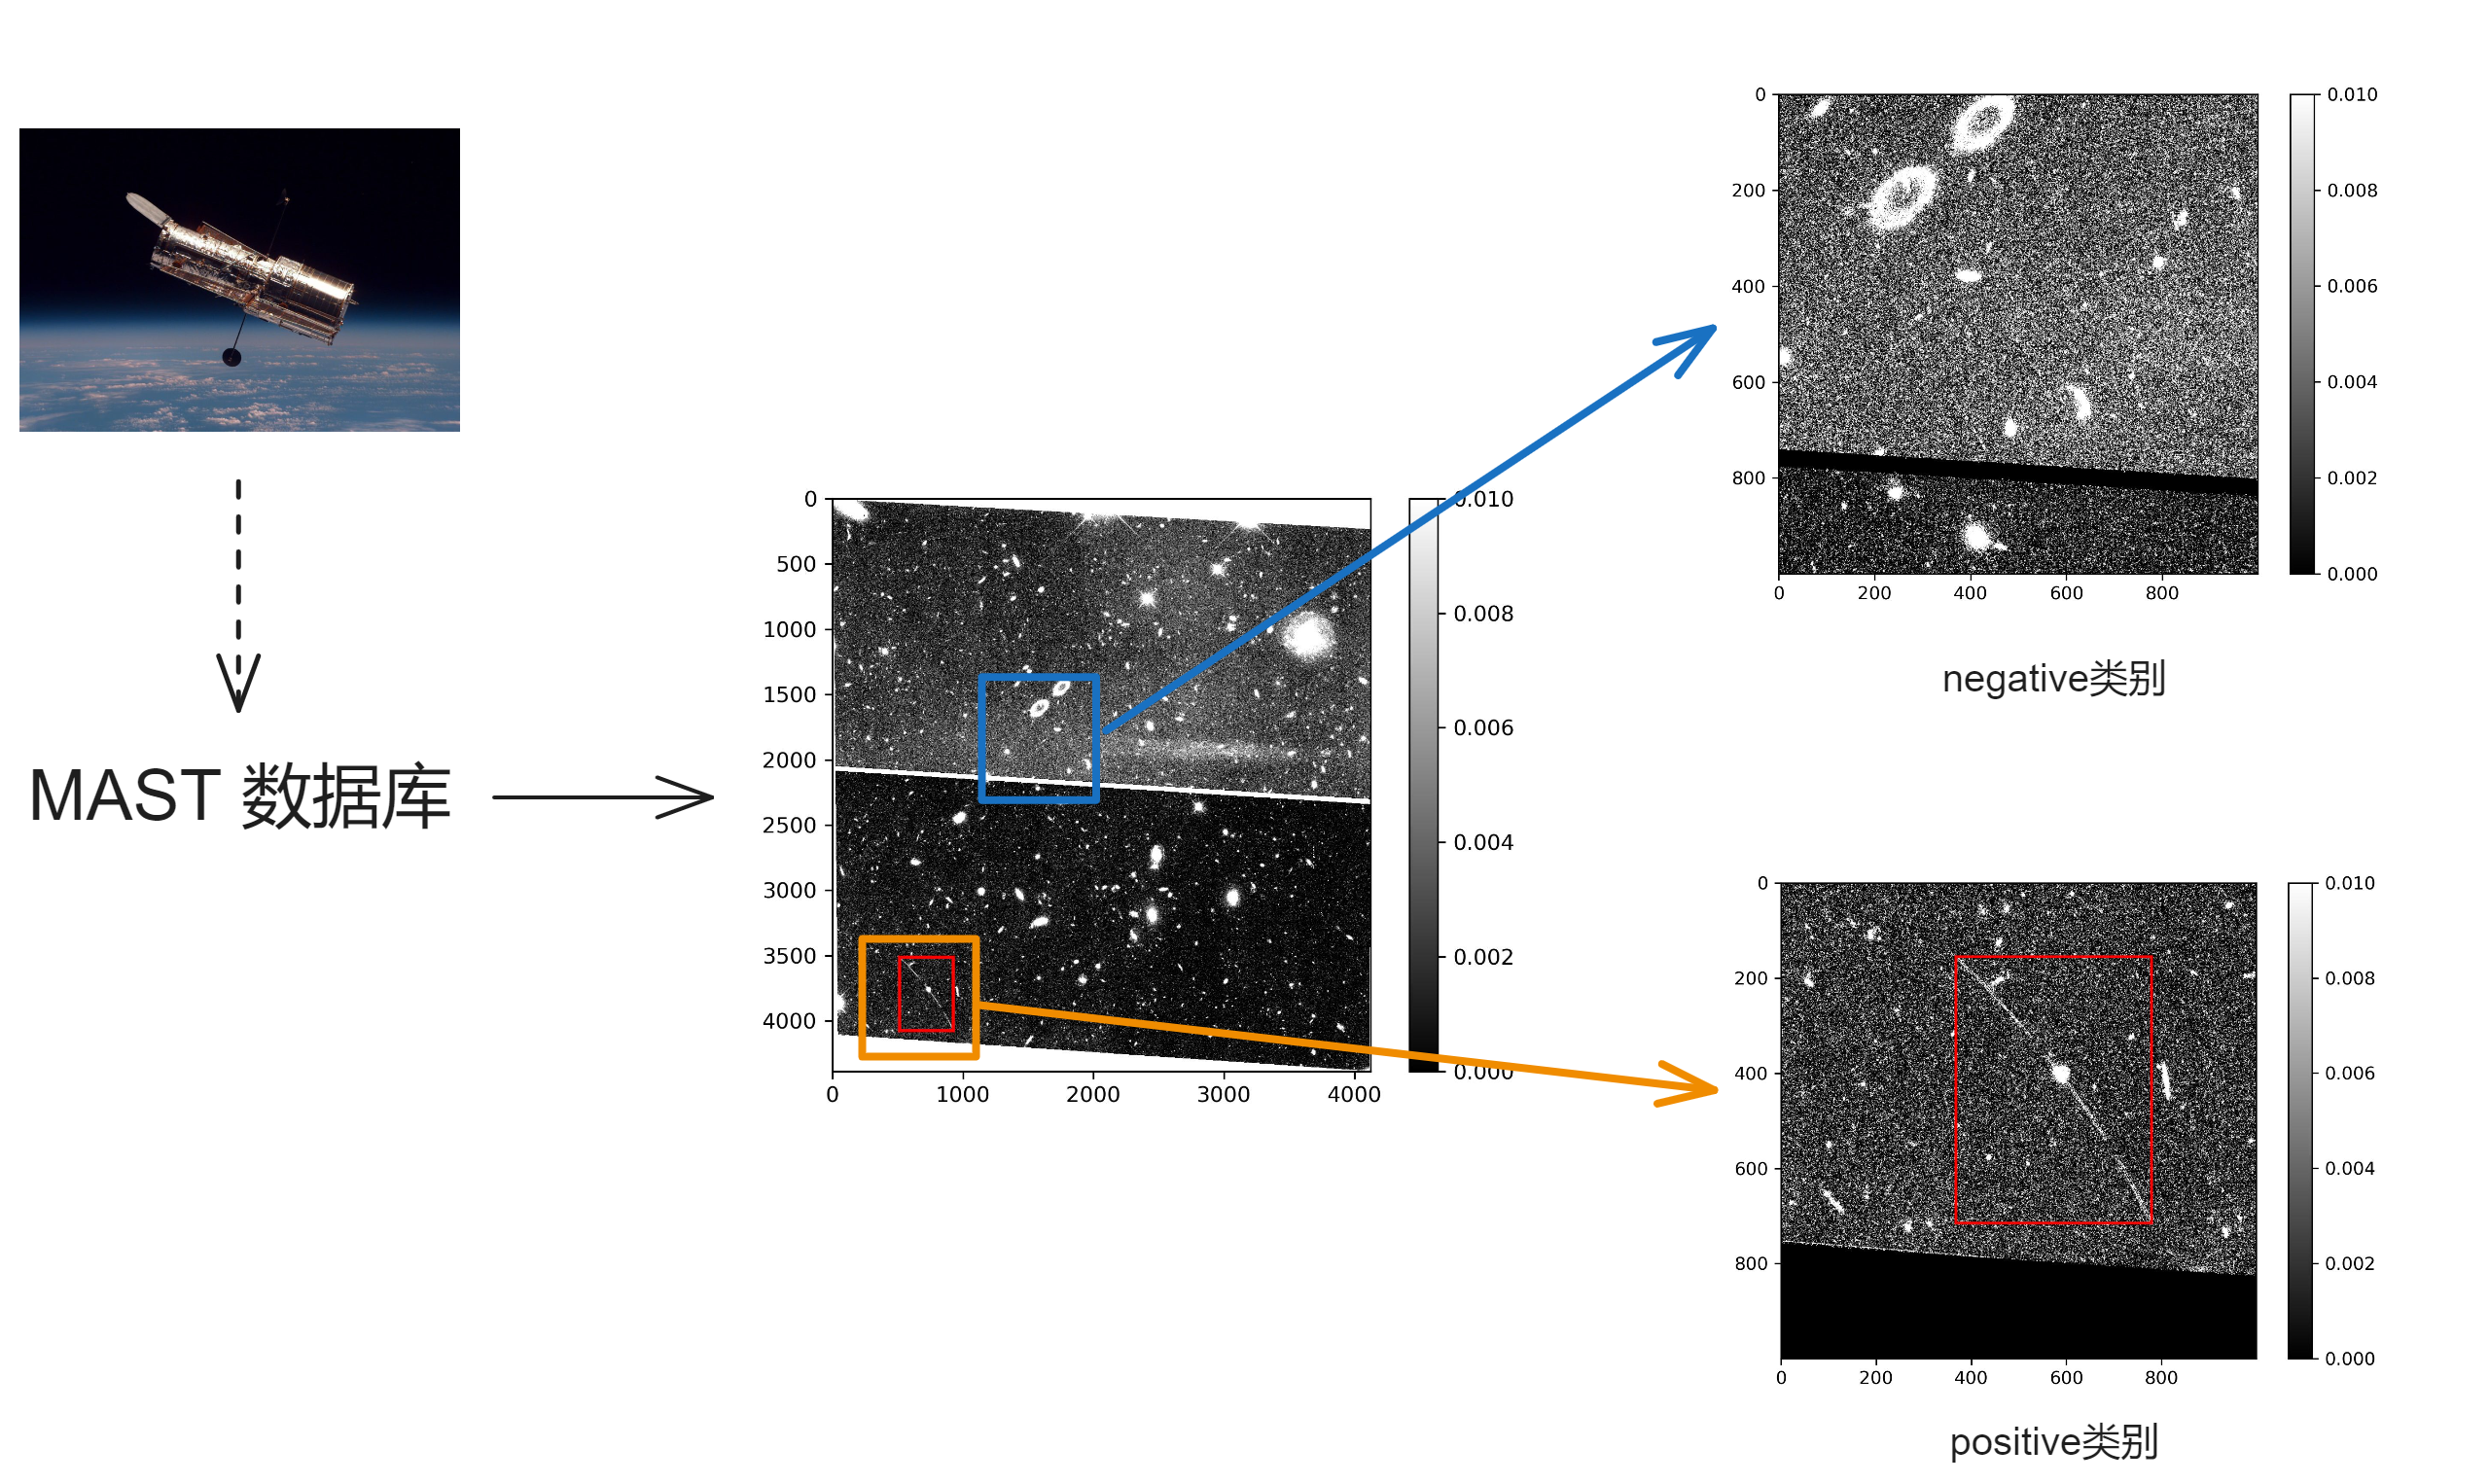
\includegraphics[width=1.0% 图片尺寸,可自行调节
            \textwidth]{preprocess.png}% 图片名称(图片需与tex文件在同一文件夹)
        \caption{\fontsize{10pt}{15pt}\selectfont 预处理流程示意图}% 图例
    \end{minipage}
\end{figure}

\subsection{训练目标}

“小行星搜索”看起来是一个目标检测问题,但实际应当被定义为一个图像分类问题。跟据文献给出的数据统计,在所有哈勃拍摄的照片中,含有一条或一条以上小行星轨迹的图像仅占总数的1.4\%,只有相当少量的照片中含有小行星轨迹目标,所以有必要优先进行分类模型的训练。

在实际操作中,我们研究了哈勃团队提供的小行星轨迹标记,发现由于小行星轨迹存在弯曲的情况,根据标记数据并不能够良好的框选出小行星的轨迹区域,训练目标检测模型的效果不佳,所以我们仅专注于提高分类模型的表现。

考虑到实际应用场景下,尽管望远镜产生了大量的图片,含有小行星的照片只占1.4\%,在已经完成高精度的分类工作后将会大大减少天文工作者人工判别的时间,这是本应用场景下的痛点问题,而进一步确定小行星轨迹位置本身不是整个任务的核心。所以,我们将“小行星搜索”转化成“图像分类问题”是符合实际应用场景需求、紧抓主要矛盾的。

综上,我们的训练目标是:将没有小行星轨迹的图像(negative类别)和有小行星轨迹的图像(positive类别)区分开。这是一个典型的二元分类问题。

\section{深度学习模型构建}

\subsection{研究背景}

近年来,随着深度学习,尤其是卷积神经网络的快速发展,越来越多的天文领域问题开始使用深度学习的方式进行解决。在图像分类领域,一系列令人振奋的成果涌现,大大提高了自动化图像分类技术的实现精度,拓宽了卷积神经网络的应用范畴。

自2012年起,出现了AlexNet, VGGNet, GoogLeNet, ResNet等一系列现代卷积神经网络,实现了在图像分类问题上跨越式的进步。AlexNet在大型数据集(如ImageNet数据集)上表现出了相比传统方法更优的性能,引领了机器视觉领域的一场革命性的进步。Simonyan et al.提出的VGGNet使用多个连续的VGG块相连,使用简单重复的网络架构实现了更深层次的卷积神经网络,进一步提升了深度学习模型在图像分类领域的表现。GoogLeNet将若干精心设计的Inception块串联起来,每个Inception使用多条并行路径,最终实现了较好的性能。残差神经网络ResNet,创造性地在VGG块的基础上,使用残差进行训练,在ImageNet数据集上展示了其出色的性能。

而在小行星发现问题上,曾经的做法往往是根据具体的观测条件下精心设计某种基于小行星物理特性的算法。这些算法本身具有高度的特化性,往往难以在不同的观测方法、观测条件中迁移。深度学习方法在不同的应用场景下都具有良好的适应性,是在小行星搜索问题上更具普遍性的解决方案。此外,随着时间的推移、观测到小行星的照片不断增加,深度学习模型可以在更大的数据集上实现更高的分类精度。

2022年,由Kruk et al.(哈勃团队成员)首次提出了结合强化学习和人工判别的方法进行自动化搜索。然而,该团队选取的模型是使用Google AutoML平台生成的目标检测模型,根据论文中提供的数据,在小行星图像分类问题上,仅实现了73.6\%的精准度(precision),58.2\%的召回率(recall),和65.0\%的F1值(f1-score)。作者没有提供开源的训练模型。尽管我们无从了解模型训练的具体细节,但显然这样的结果存在较大的优化空间。Cowan et al.在2023年初将深度学习算法用于MOA微引力透镜巡天数据库上,给出了一套地面望远镜观测数据处理的解决方案,实现了较好的小行星搜索结果。遗憾的是,由于作者使用的标记数据集和预处理步骤并不公开,我们暂时无法在同样的数据库上复现作者的成果或进行二次开发。

本文提出使用迁移学习的方式,对预训练模型进行微调训练,以适应我们选取的哈勃望远镜图像分类任务。我们从公开数据库中构建数据集,通过微调训练实现优异的分类精度,希望能为今后的小行星搜索工作提供可以直接迁移借鉴的成果,提供一些启发。

\subsection{模型构建方法}

考虑到我们的数据集体量相对较小,直接从零训练成本高且容易过拟合,我们提出使用预训练模型进行迁移学习的方法来减少训练时间并提高训练成果精度。我们使用Pytorch深度学习框架完成模型构建代码,使用torchvision第三方库中的预训练参数进行迁移训练。这些参数是经典的图像分类模型在ImageNet数据集上训练的成果。

为使得模型能够更好地进行深度学习训练,我们首先将所有图像(NumPy Array格式)归一化到0至1之间;然后将NumPy Array格式的数据转换成PIL图像,并将图片尺寸设置为224*224,符合预训练模型在ImageNet数据集上训练时的尺寸;接着,将训练集图片进行随机水平翻转;最后,将PIL格式的图片转换成tensor格式并完成DataLoader构建。

不同于ImageNet数据集中的RGB三通道图像,我们从哈勃获取的图像是单通道的灰度图,所以在进行迁移训练的时候需要重新设计第一个卷积层。在此过程中,我们选取的方法是将三通道修改为单通道,微调的初始权重取原先RGB三个通道的平均值。在这种情况下,我们成功将原本的预训练模型适配到现有的数据集。此外,模型本身是在ImageNet数据集上训练的,所以输出数量是1000类。而我们现在的分类问题是简单的二元分类,还需要将原先的输出层的输出数量设置为2并进行参数随机初始化。

\begin{figure}[H]% 插入一张图片,H表示浮动环境下的here
    \centering
    \begin{minipage}{0.65\textwidth}% 小页面尺寸,可自行调节
        \centering
        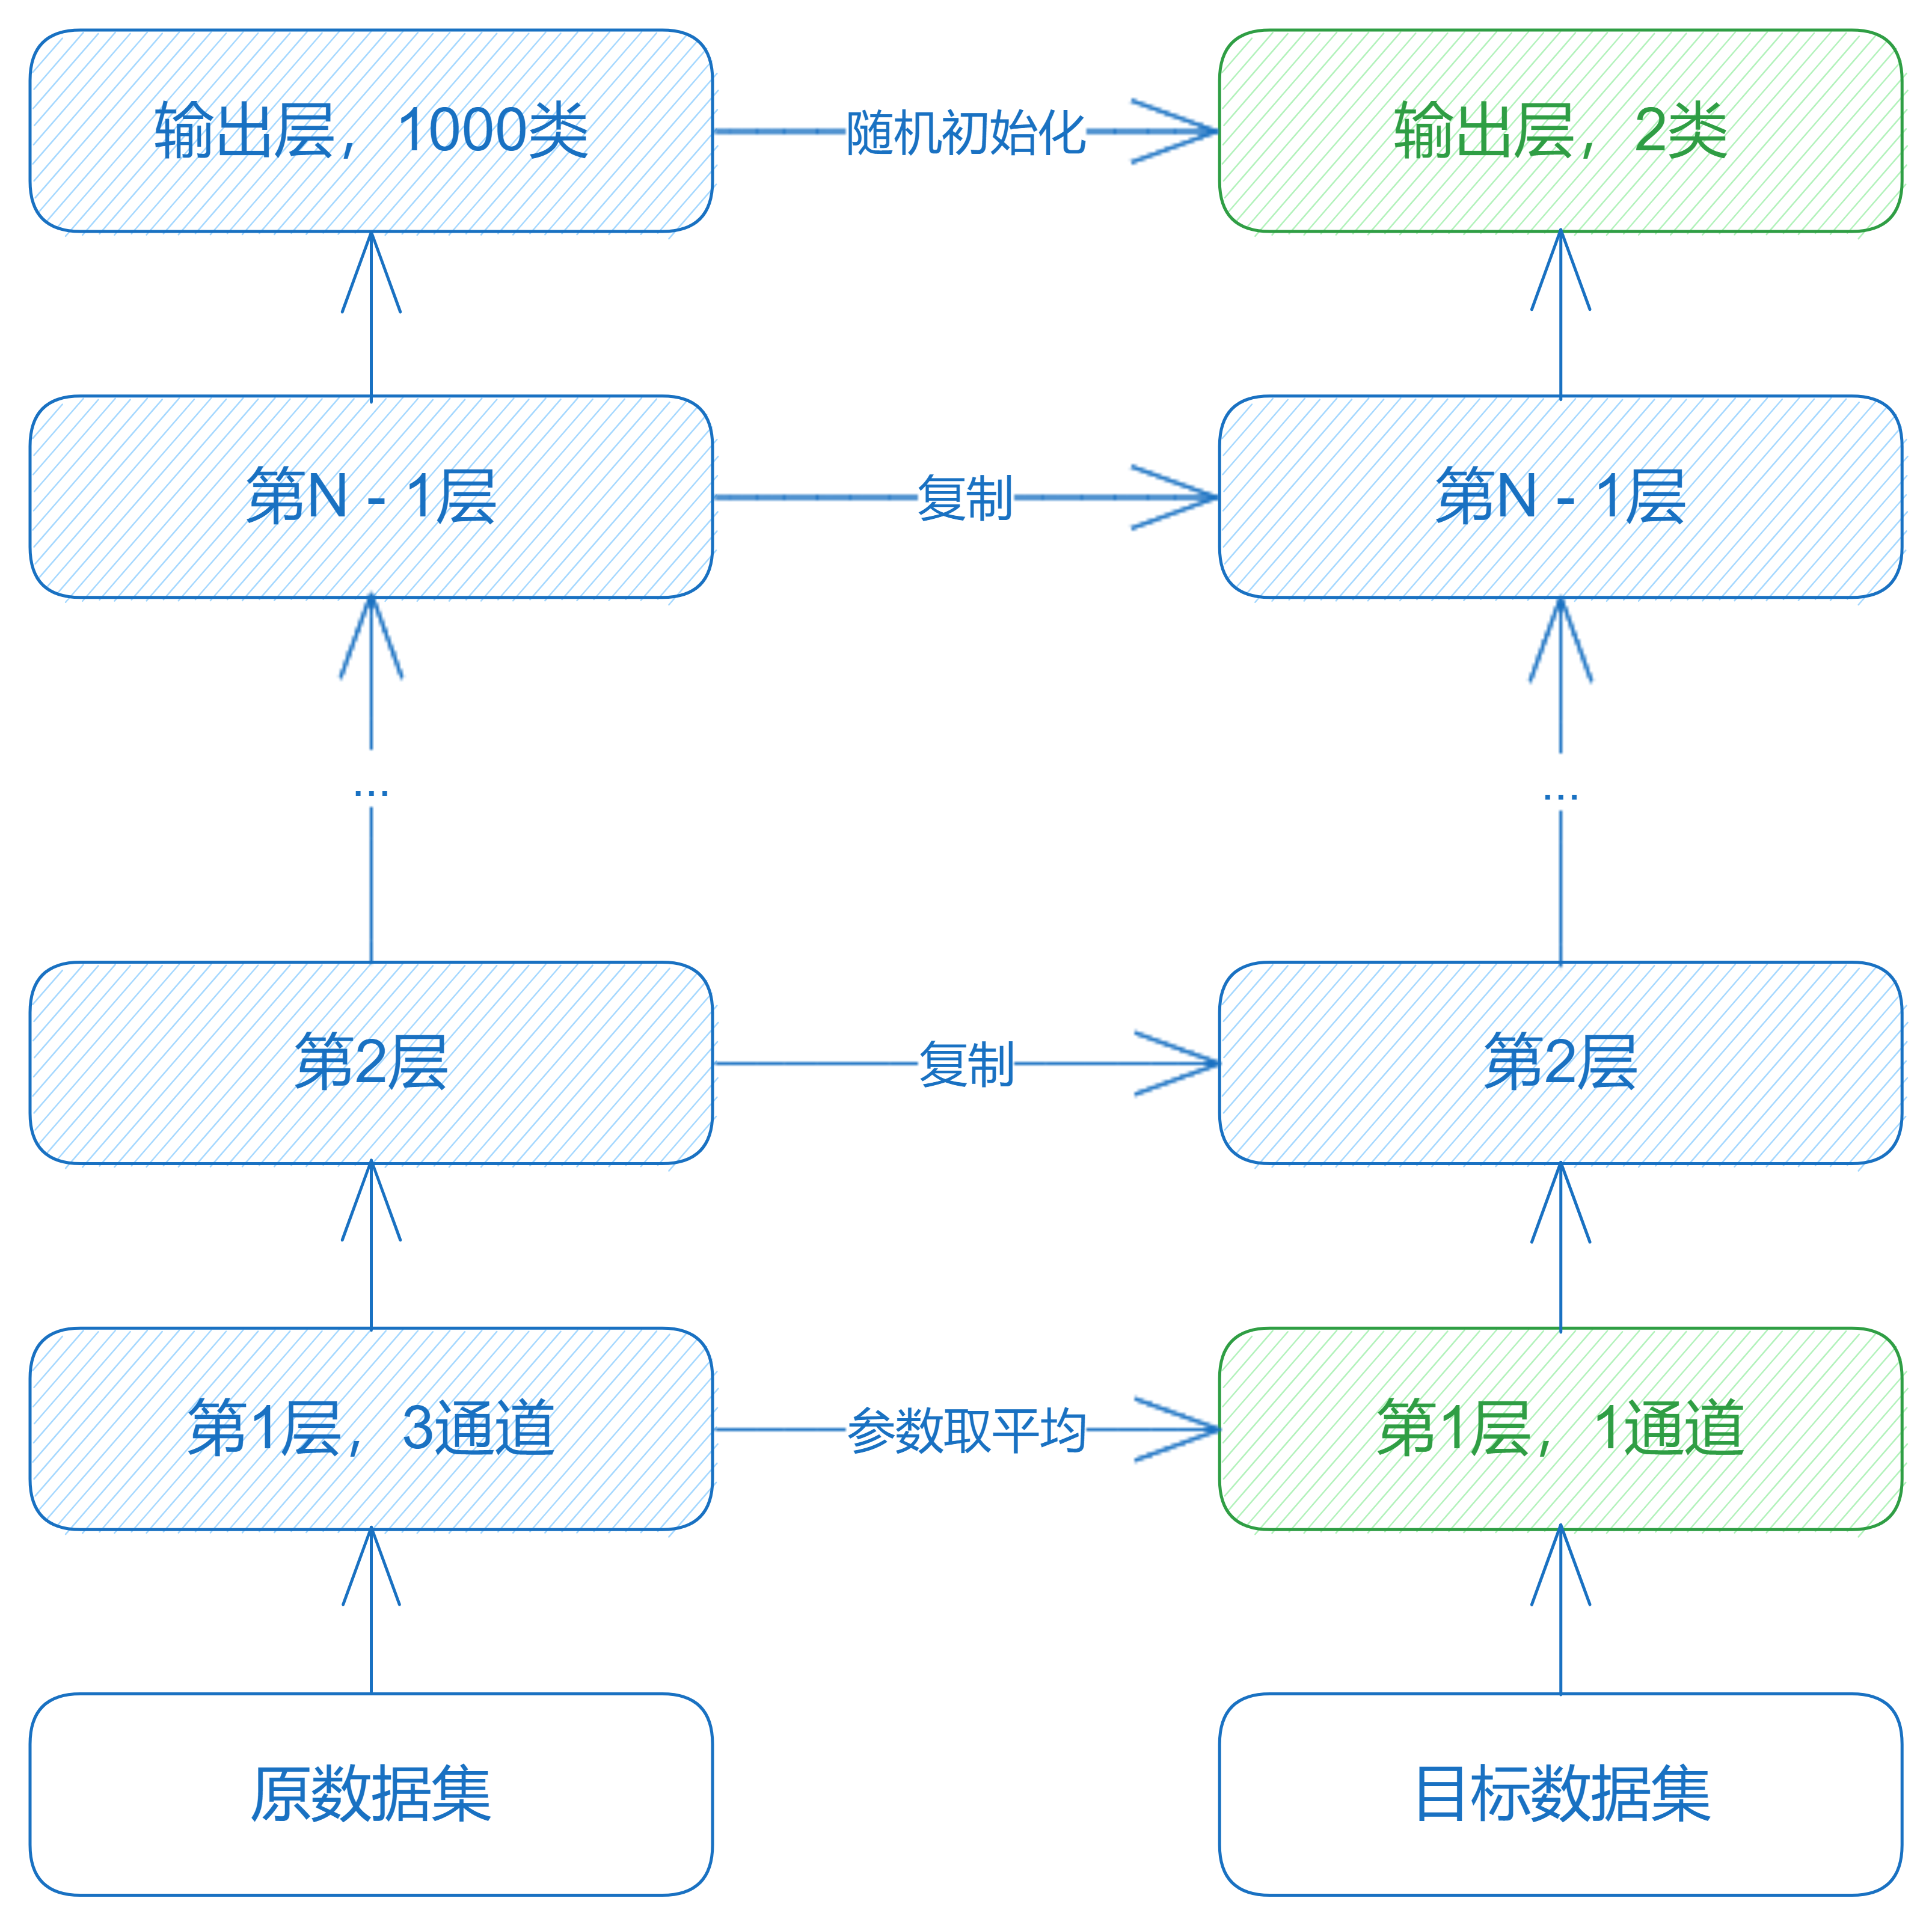
\includegraphics[width=1.0% 图片尺寸,可自行调节
            \textwidth]{fine-tune.png}% 图片名称(图片需与tex文件在同一文件夹)
        \caption{\fontsize{10pt}{15pt}\selectfont 微调模型构建示意图}% 图例
    \end{minipage}
\end{figure}

\subsection{训练模型}

在设定好模型初始参数后,下一步就要进行迁移模型训练。我们挑选了经典的ResNet系列和VGG系列模型进行迁移训练。其中,ResNet系列选用的模型为ResNet18,ResNet34,ResNet50和ResNet101;VGG系列选用的模型为VGG16,VGG19。

经过一系列尝试,我们最终设定Batch Size为4,epoch数量为25,选择使用SGD作为优化器,设定初始学习率为0.001并且每7个epoch学习率降低为原来的0.1倍,使用CrossEntropy作为损失函数,以此为基础进行训练。

由于条件有限,我们在一台配置了RTX 2050显卡的PC电脑上进行训练,使用Pytorch版本为2.0.1。最终,我们数据集的大小为positive类别1696张,negative类别1586张。

在训练过程中,每个epoch使用训练集进行训练,然后通过检测集获得检测分数,最后选取检测分数最高的模型预测测试集并得到最终的结果。

\section{结果和讨论}

经过训练,我们得出的结果如表中所示(Table 2)。

ResNet系列模型中表现最好、准确率最高的模型是ResNet50。从ResNet18到ResNet50,随着卷积神经网络的加深,Accuracy的数值的确在不断提高,但是当ResNet深度提高到101个卷积层时反而表现下降,似乎在本应用场景下,过深的残差网络反而对整体预测性能有害无益。

\begin{table}[H]% 插入表格
    \centering
    \caption{\fontsize{10pt}{15pt}\selectfont Hubble Asteroid Hunter数据集样例}
    \begin{tabular}{ccccc}
        \toprule[1.5pt]
        预训练模型     & Accuracy & Precision & Recall & F1-score \\

        \midrule
        ResNet18  & 0.9041   & 0.8971    & 0.9083 & 0.9027   \\
        ResNet34  & 0.9143   & 0.9459    & 0.8750 & 0.9091   \\
        ResNet50  & 0.9224   & 0.9280    & 0.9125 & 0.9202   \\
        ResNet101 & 0.8918   & 0.9193    & 0.8542 & 0.8855   \\
        VGG16     & 0.9122   & 0.9087    & 0.9125 & 0.9106   \\
        \bottomrule[1.5pt]
    \end{tabular}
\end{table}


\section{研究价值及创新点}

在我们了解的现有研究中,我们是首个将完备的深度学习图像分类技术应用在哈勃空间望远镜公开数据库上的。通过科学的迁移训练方法和完备的实验,我们将小行星搜索工作的自动化程度大大增加,将显著减少相关领域工作者的工作量,提高整体小行星发现效率。

不同于以往研究,我们的工作实现了从数据集构建到模型训练完全使用公开资源,今后在本领域的研究可以非常轻松地借助本研究的成果进行复现、优化和迁移。总之,本文对人类了解太阳系环境、确保地球自身安全有一定积极作用。

\section{总结和展望}

本文证明了将深度学习方法应用在哈勃数据库中进行小行星搜索是完全可行的。尽管我们选用的训练数据集偏小,我们仍然能够通过微调预训练模型的方法,实现相当好的分类效果。在所有模型中,我们实现了最大准确率(Accuracy)达到92.24\%,最大召回率达91.25\%,结果基本令人满意。

我们设计了一套自动化批处理流水线,实现从数据下载、预处理到模型训练的完全自主处理,且该流水线具有相当的可迁移性,稍加改进即可运用在哈勃之外的其他望远镜的数据库中,对今后的天文观测工作有一定的借鉴意义。

下一步,我们希望进一步提高训练准确率,重点提高模型的召回率,尽可能确保所有数据库中捕获的小行星都被发现、处理;

我们希望通过人工重新标记数据,提高数据集标记质量,完成“图像分类+目标检测”全流程训练,在现有基础上进一步降低天文工作者的工作量,提高小行星发现效率;

我们希望能够进一步复合天文领域专业软件,实现小行星轨道自动解算、自动判别是否为太阳系内天体,乃至于自动将未知小行星数据自动报送给国际天文联合会(IAU)的小行星中心(Minor Planet Center, MPC),实现更高程度的自动化;

此外,我们还会将训练好的模型直接应用在哈勃数据库当中,力求从哈勃天文望远镜的海量数据中提取出仍然未被发现的小行星并报送给MPC,为人类生存环境的安全贡献自己的力量。



\newpage

\bibliographystyle{unsrt}
\bibliography{bh2}

\newpage

\section*{致谢}

我们是三位天文爱好者,技术爱好者。这篇文章的想法来源于我们参与公众科学项目IASC时的亲身感受。在IASC项目中,参与的志愿者还需要用肉眼找小行星,显得不是特别优雅,所以我们想到了或许可以把时下最火的深度学习技术应用到该领域。事实表明,这种想法完全是可行的。

在项目中,孙畅负责了整体工作统筹安排、数据预处理、模型构建和训练,参与了模型超参数调优和论文撰写;邹桐负责了超参数调优,参与了数据预处理和模型构建;周佳颖负责了论文撰写工作,参与了数据预处理工作。整个研究的绝大多数工作完全是由我们三人合作完成的。

我们要感谢我校的史镨镭老师。史老师是我们的信息课老师,在论文选题、前置知识学习方面为我们提供了悉心指导。论文的结构和内容都是由我们三位同学完成的,史老师在初稿成文后就文字组织方面提供一定的修改建议。史老师对我们的指导工作是无偿的。此外,整个研究中不含有他人协助完成的成果。

总之,这次研究极大地锻炼了我们的深度学习技术应用能力。我们三位同学对自己能够完全凭借自身力量完成几乎全部研究而感到骄傲!

\end{document}% 结束文档编辑,后面写啥都编译不出来